\documentclass[a4paper,12pt]{extarticle}
%Gummi|065|=)
\usepackage[T1]{fontenc}
\usepackage[utf8]{inputenc}
\usepackage[russian]{babel}
\usepackage[left=3cm,right=1.5cm,
    top=2cm,bottom=2cm,bindingoffset=0cm]{geometry}
\usepackage{amsmath}
\usepackage{caption}
% \usepackage{color}
\usepackage{graphicx}
\usepackage{enumitem}
\usepackage{verbatimbox}
\usepackage{verbatim}
\usepackage{xcolor}
\usepackage{fancyvrb}
\usepackage{indentfirst}
\usepackage{alltt}

\usepackage[cache=false]{minted}
\usepackage{tcolorbox}
\usepackage{etoolbox}
\BeforeBeginEnvironment{minted}{\begin{tcolorbox}}%
\AfterEndEnvironment{minted}{\end{tcolorbox}}%

\linespread{1.3}
\begin{document}

% НАЧАЛО ТИТУЛЬНОГО ЛИСТА

    \begin{table}[h!]
     \begin{center}
     \begin{tabular}{  c  p{0.8\textwidth}  }
     \raisebox{-\totalheight}{
\includegraphics[width=0.15\textwidth, height=30mm]{bmstu.png}}
      & 
      \begin{center}
          Министерство образования и науки Российской Федерации \\
      Федеральное государственное бюджетное образовательное учреждение высшего образования  \\
    
      «Московский государственный технический университет \\
      имени Н.Э. Баумана» \\
    
      (МГТУ им. Н.Э. Баумана)
      \end{center}
      \\
      \hline
      \end{tabular}
      \end{center}
\end{table}

\textbf{ }
\\
\textbf{ФАКУЛЬТЕТ: } \underline{Информатика и системы управления}
\\
\textbf{КАФЕДРА: } \underline{Программное обеспечение ЭВМ и информационные технологии}
\\
\textbf{ДИСЦИПЛИНА: } \underline{Типы и структуры данных}
\\
\textbf{ТЕМА: } \underline{Обработка деревьев и хеш-таблиц
}
\\
\textbf{ВАРИАНТ: } \underline{3}

\vspace{1cm}

\begin{center}
    \large{\textbf{\underline{ОТЧЕТ ПО ЛАБОРАТОРНОЙ РАБОТЕ №6}}}
\end{center}

\textbf{ }
\vspace{1cm}
\\
\textbf{Студент: } \hspace{5.2cm} \underset{\text{(подпись, дата)}}{\underline{\hspace{0.3\textwidth}}} \textit{ Княжев А. В. }
\vspace{0.2cm}
\\
\textbf{Преподаватель: } \hspace{4cm} \underset{\text{(подпись, дата)}}{\underline{\hspace{0.3\textwidth}}} \textit{ Силантьева А. В. }

\vspace{7cm}
\begin{center} \textit{2021 г.} \end{center}
\thispagestyle{empty}
\newpage

\tableofcontents
\newpage

\section{Условие задачи}

Построить ДДП, в вершинах которого находятся слова из текстового файла. Вывести его на экран в виде дерева. Сбалансировать полученное дерево и вывести его на экран. Удалить указанное слово в исходном и сбалансированном дереве. Сравнить время удаления и объем памяти. Построить хеш-таблицу из слов текстового файла, задав размерность таблицы с экрана, используя метод цепочек для устранения коллизий. Вывести построенную таблицу слов на экран. Осуществить удаление введенного слова, вывести таблицу. Сравнить время удаления, объем памяти и количество сравнений при использовании ДДП, сбалансированных деревьев, хеш-таблиц и файла.

\newpage

\section{Техническое задание}

Построить дерево в соответствии с заданным вариантом задания. Вывести его на экран в виде дерева. Реализовать основные операции работы с деревом: обход дерева, включение, исключение и поиск узлов. Сравнить эффективность алгоритмов сортировки и поиска в зависимости от высоты дерева и степени его ветвления. Построить хеш-таблицу по указанным данным. Вывести на экран деревья и хеш-таблицу. Сравнить эффективность поиска в двоичном дереве поиска, в сбалансированном дереве поиска и в хеш-таблице. Вывести на экран измененные структуры. Подсчитать среднее количество сравнений для поиска данных в указанных структурах. Произвести реструктуризацию хеш-таблицы, если среднее количество сравнений больше указанного. 

Оценить эффективность использования этих структур (по времени и памяти) для поставленной задачи.

Программа должна выводить меню с возможностью выбирать варианты. При вводе нуля на запрос варианта меню, происходит выход из программы.

\subsection{Общие входные данные}
\begin{itemize}
	\item[$*$] имя файла со словами;
	\item[$*$] емкость хеш-таблицы;
    \item[$*$] номер выбранного пункта меню.
\end{itemize}

\subsection{Входные и выходные данные пунктов меню}
\subsubsection{Вывод ДДП}

\paragraph{Выходные данные}
\begin{itemize}
    \item[$*$] текстовый файл с описанием дерева;
    \item[$*$] графическое изображение дерева.
\end{itemize}

\subsubsection{Поиск элемента в ДДП}

\paragraph{Входные данные}
\begin{itemize}
    \item[$*$] строка --- элемент, который ищется в ДДП.
\end{itemize}

\paragraph{Выходные данные}
\begin{itemize}
    \item[$*$] сообщение о найденном элементе;
    \item[$*$] время выполнения операции.
\end{itemize}

\subsubsection{Удаление элемента из ДДП}

\paragraph{Входные данные}
\begin{itemize}
    \item[$*$] строка --- удаляемый элемент.
\end{itemize}

\paragraph{Выходные данные}
\begin{itemize}
    \item[$*$] сообщение об успешном удалении;
    \item[$*$] время выполнения операции.
\end{itemize}

\subsubsection{Вывод АВЛ-дерева}

\paragraph{Выходные данные}
\begin{itemize}
    \item[$*$] текстовый файл с описанием дерева;
    \item[$*$] графическое изображение дерева.
\end{itemize}


\subsubsection{Поиск элемента в АВЛ-дереве}

\paragraph{Входные данные}
\begin{itemize}
    \item[$*$] строка --- элемент, который ищется в АВЛ-дереве.
\end{itemize}

\paragraph{Выходные данные}
\begin{itemize}
    \item[$*$] сообщение о найденном элементе;
    \item[$*$] время выполнения операции.
\end{itemize}

\subsubsection{Удаление элемента из АВЛ-дерева}

\paragraph{Входные данные}
\begin{itemize}
    \item[$*$] строка --- удаляемый элемент.
\end{itemize}

\paragraph{Выходные данные}
\begin{itemize}
    \item[$*$] сообщение об успешном удалении;
    \item[$*$] время выполнения операции.
\end{itemize}

\subsubsection{Вывод хеш-таблицы}

\paragraph{Входные данные}

\paragraph{Выходные данные}
\begin{itemize}
    \item[$*$] элементы хеш-таблицы в формате \texttt{<index> <key>}.
\end{itemize}

\subsubsection{Поиск элемента в хеш-таблице}

\begin{itemize}
    \item[$*$] строка --- элемент, который ищется в хеш-таблице.
\end{itemize}

\paragraph{Выходные данные}
\begin{itemize}
    \item[$*$] сообщение о найденном элементе;
    \item[$*$] время выполнения операции.
\end{itemize}

\subsubsection{Удаление элемента из хеш-таблицы}

\paragraph{Входные данные}
\begin{itemize}
    \item[$*$] строка --- удаляемый элемент.
\end{itemize}

\paragraph{Выходные данные}
\begin{itemize}
    \item[$*$] сообщение об успешном удалении;
    \item[$*$] время выполнения операции.
\end{itemize}

\subsubsection{Сравнение скорости}

\paragraph{Входные данные}
\begin{itemize}
    \item[$*$] количество элементов в сравниваемых структурах;
    \item[$*$] емкость хеш-таблицы.
\end{itemize}

\paragraph{Выходные данные}
\begin{itemize}
    \item[$*$] скорость поиска и удаления для:
    \begin{enumerate}
    	\item ДДП;
    	\item АВЛ-дерева;
    	\item хеш-таблицы;
    	\item текстового файла.
    \end{enumerate}
\end{itemize}

\subsubsection{Сравнение потребления памяти}

\paragraph{Входные данные}
\begin{itemize}
    \item[$*$] количество элементов в сравниваемых структурах;
    \item[$*$] емкость хеш-таблицы.
\end{itemize}

\paragraph{Выходные данные}
\begin{itemize}
    \item[$*$] объем памяти, занимаемый:
    \begin{enumerate}
    	\item ДДП;
    	\item АВЛ-деревом;
    	\item хеш-таблицей.
    \end{enumerate}
\end{itemize}

\subsection{Действие программы}
Программа осуществляет работу с двоичными деревьями поиска, сбалансированными деревьями и хеш-таблицами.

\subsection{Обращение к программе}
Программа может быть запущена из командных оболочек \texttt{sh/bash/zsh/fish}, а также от IDE, способных работать с языком Си. Программа не принимает никаких аргументов. Название исполняемого файла --- app.exe, так что команда может быть вызвана из командной оболочки в корневой папке проекта как:

\begin{minted}{bash}
$ ./app.exe
\end{minted}

\subsection{Аварийные ситуации}
\subsubsection{Общие аварийные ситуации}
\begin{enumerate}
	\item файл со словами не существует;
	\item файл со словами пуст;
	\item строка, содержащая имя файла слишком длинная;
	\item невалидая емкость хеш-таблицы;
	\item некорректная емкость хеш-таблицы;
    \item невалидный номер пункта меню (строка или пустая строка);
    \item неверный номер пункта меню (такого пунта меню не существует).
\end{enumerate}

\subsubsection{Пункт меню №1}
\begin{enumerate}
    \item дерево пусто.
\end{enumerate}

\subsubsection{Пункт меню №2}
\begin{enumerate}
    \item введенная строка поиска слишком длинная.
\end{enumerate}

\subsubsection{Пункт меню №3}
\begin{enumerate}
    \item введенная удаляемая строка слишком длинная.
\end{enumerate}

\subsubsection{Пункт меню №4}
\begin{enumerate}
    \item дерево пусто.
\end{enumerate}

\subsubsection{Пункт меню №5}
\begin{enumerate}
    \item введенная строка поиска слишком длинная.
\end{enumerate}

\subsubsection{Пункт меню №6}
\begin{enumerate}
    \item введенная удаляемая строка слишком длинная.
\end{enumerate}

\subsubsection{Пункт меню №7}
\begin{enumerate}
    \item хеш-таблица пуста.
\end{enumerate}

\subsubsection{Пункт меню №8}
\begin{enumerate}
    \item введенная строка поиска слишком длинная.
\end{enumerate}

\subsubsection{Пункт меню №9}
\begin{enumerate}
    \item введенная удаляемая строка слишком длинная.
\end{enumerate}

\subsubsection{Пункт меню №10}
\begin{enumerate}
    \item невалидное количество элементов;
    \item некорректное количество элементов;
    \item невалидная емкость хеш-таблицы;
    \item некорректная емкость хеш-таблицы.
\end{enumerate}

\subsubsection{Пункт меню №11}
\begin{enumerate}
    \item невалидное количество элементов;
    \item некорректное количество элементов;
    \item невалидная емкость хеш-таблицы;
    \item некорректная емкость хеш-таблицы.
\end{enumerate}

\newpage

\section{Структуры данных}
В данной работе используется динамические массивы, записи, односвязные списки, деревья.

\subsection{Модуль для работы двоичным деревом поиска}
\subsubsection{Типы данных}

\begin{minted}{C}
/**
 * Двоичное дерево поиска (ДДП).
 * key - ключ (слово);
 * left - указатель на левого потомка;
 * right - указатель на правого потомка.
 */
typedef struct bst_t bst_t;
struct bst_t
{
    mystring_t key;
    bst_t *left;
    bst_t *right;
};
\end{minted}

\subsubsection{Функции}

\begin{minted}{C}
/**
 * Вставка элемента в ДДП.
 * root - корень исходного дерева;
 * key - вставляемый ключ (слово).
 */
error_t bst_insert(bst_t **root, mystring_t key);
\end{minted}


\begin{minted}{C}
/**
 * Освобождение ДДП.
 * root - корень исходного дерева.
 */
void bst_free(bst_t **root);
\end{minted}


\begin{minted}{C}
/**
 * Вывод ДДП на экран в виде изображения.
 * root - корень исходного дерева.
 */
error_t bst_show(bst_t **root);
\end{minted}


\begin{minted}{C}
/**
 * Удаление элемента из ДДП.
 * root - корень исходного дерева;
 * key - удаляемый ключ (слово).
 */
error_t bst_remove(bst_t **root, mystring_t key);
\end{minted}


\begin{minted}{C}
/**
 * Чтение ДДП из файла.
 * root - корень исходного дерева;
 * f - файл.
 */
error_t bst_from_file(bst_t **root, FILE *f);
\end{minted}


\begin{minted}{C}
/**
 * Поиск элемента в ДДП.
 * root - корень исходного дерева;
 * key - искомый ключ (слово);
 * result - найденный узел.
 */
error_t bst_search(bst_t **root, mystring_t key, bst_t **result);
\end{minted}


\subsection{Модуль для работы с АВЛ-деревом}

\subsubsection{Типы данных}

\begin{minted}{C}
/**
 * АВЛ-дерево.
 * key - ключ (слово);
 * height - высота текущего узла;
 * left - указатель на левого потомка;
 * right - указатель на правого потомка.
 */
typedef struct avl_t avl_t;
struct avl_t
{
    mystring_t key;
    int height;
    avl_t *left;
    avl_t *right;
};
\end{minted}

\subsubsection{Функции}

\begin{minted}{C}
/**
 * Вставка элемента в АВЛ-дерево.
 * root - корень исходного дерева;
 * key - вставляемый ключ (слово).
 */
error_t avl_insert(avl_t **root, mystring_t key);
\end{minted}


\begin{minted}{C}
/**
 * Освобождение АВЛ-дерева.
 * root - корень исходного дерева.
 */
void avl_free(avl_t **root);
\end{minted}


\begin{minted}{C}
/**
 * Вывод АВЛ-дерева на экран в виде изображения.
 * root - корень исходного дерева.
 */
error_t avl_show(avl_t **root);
\end{minted}


\begin{minted}{C}
/**
 * Удаление элемента из АВЛ-дерева.
 * root - корень исходного дерева;
 * key - удаляемый ключ (слово).
 */
error_t avl_remove(avl_t **root, mystring_t key);
\end{minted}


\begin{minted}{C}
/**
 * Чтение АВЛ-дерева из файла.
 * root - корень исходного дерева;
 * f - файл.
 */
error_t avl_from_file(avl_t **root, FILE *f);
\end{minted}


\begin{minted}{C}
/**
 * Поиск элемента в АВЛ-дереве.
 * root - корень исходного дерева;
 * key - искомый ключ (слово);
 * result - найденный узел.
 */
error_t avl_search(avl_t **root, mystring_t key, avl_t **result);
\end{minted}


\subsection{Модуль для работы с хеш-таблицей}

\subsubsection{Типы данных}

\begin{minted}{C}
/**
 * Список-элемент хеш-таблицы.
 * key - ключ (слово);
 * next - указатель на следующий элемент списка.
 */
typedef struct ht_element_t ht_element_t;
struct ht_element_t
{
    mystring_t key;
    ht_element_t *next;
};
\end{minted}

\begin{minted}{C}
/**
 * Хеш-таблица.
 * table - элементы таблицы (списки);
 * size - емкость хеш-таблицы;
 * hash - функция хеширования.
 */
typedef struct ht_t
{
    ht_element_t **table;
    size_t size;
    size_t (*hash) (mystring_t, size_t);
} ht_t;
\end{minted}

\subsubsection{Функции}

\begin{minted}{C}
/**
 * Создание новой хеш-таблицы.
 * size - емкость хеш-табицы;
 * hash - функция хеширования.
 */
ht_t *ht_new(size_t size, size_t (*hash) (mystring_t, size_t));
\end{minted}

\begin{minted}{C}
/**
 * Освобождение хеш-таблицы.
 * ht - исходная хеш-таблица.
 */
void ht_free(ht_t **ht);
\end{minted}

\begin{minted}{C}
/**
 * Вставка слова в хеш-таблицу.
 * ht - исходная хеш-таблица;
 * key - вставляемый ключ (слово).
 */
error_t ht_insert(ht_t **ht, mystring_t key);
\end{minted}

\begin{minted}{C}
/**
 * Удаление элемента из хеш-таблицы.
 * ht - исходная хеш-таблица;
 * key - удаляемый ключ (слово).
 */
error_t ht_remove(ht_t **ht, mystring_t key);
\end{minted}

\begin{minted}{C}
/**
 * Поиск элемента в хеш-таблице.
 * ht - исходная хеш-таблица;
 * key - искомый ключ;
 * found - найденный элемент.
 */
error_t ht_search(ht_t **ht, mystring_t key, ht_element_t **found);
\end{minted}

\begin{minted}{C}
/**
 * Вывод хеш-таблицы.
 * ht - исходная хеш-таблица.
 */
error_t ht_print(ht_t **ht);
\end{minted}

\begin{minted}{C}
/**
 * Ввод хеш-таблицы из файла.
 * ht - исходная хеш-таблица;
 * f - файл.
 */
error_t ht_from_file(ht_t **ht, FILE *f);
\end{minted}

\begin{minted}{C}
/**
 * Аддитивная хеш-функция.
 * str - преобразуемая строка;
 * size - емкость хеш-таблицы.
 */
size_t ht_additive_method(mystring_t str, size_t size);
\end{minted}


\subsection{Модуль для работы с текстовым файлом}

\subsubsection{Функции}

\begin{minted}{C}
/**
 * Добавление слова в текстовый файл.
 * filename - имя файла;
 * key - добавляемое слово.
 */
error_t file_insert(char *filename, mystring_t key);
\end{minted}

\begin{minted}{C}
/**
 * Удаление слова из текстового файла.
 * filename - имя файла;
 * key - удаляемое слово.
 */
error_t file_remove(char *filename, mystring_t key);
\end{minted}

\begin{minted}{C}
/**
 * Поиск слова в текстовом файле.
 * filename - имя файла;
 * key - искомое слово.
 */
error_t file_search(char *filename, mystring_t key);
\end{minted}


\subsection{Модуль для работы с ошибками}
\subsubsection{Типы данных}
\begin{minted}{C}
/**
 * text - текст ошибки;
 * code - код ошибки;
 * func - функция, в которой случилась ошибка.
 */
typedef struct 
{
    const char *text;
    int code;
    const char *func;
} error_t;
\end{minted}


\subsubsection{Функции}
\begin{minted}{C}
/**
 * Создание новой ошибки.
 * text - текст ошибки;
 * code - код ошибки;
 * func - функция, в которой случилась ошибка.
 */
error_t new_error(const char *text, int code, const char *func);
\end{minted}


\begin{minted}{C}
/**
 * Создание ошибки-маркера успеха.
 * func - функция, в которой был создан "успех".
 */
error_t new_success(const char *func);
\end{minted}



\begin{minted}{C}
/**
 * Проверка, отображает ли ошибка ошибочную ситуацию.
 * err - исходная ошибка.
 */
bool is_failure(error_t err);
\end{minted}


\subsection{Модуль для работы со строками}
\subsubsection{Основные константы}
\begin{minted}{C}
#define MYSTRING_SIZE 257
\end{minted}


\subsubsection{Типы данных}
\begin{minted}{C}
/**
 * Тип строки длиной 256 символов + терминальный нуль.
 */
typedef char mystring_t[MYSTRING_SIZE];
\end{minted}

\subsubsection{Функции}
\begin{minted}{C}
/**
 * Чтение строки из файла.
 * f - файл;
 * str - строка, в которую считываем.
 */
error_t ms_read_line(FILE *f, mystring_t str);
\end{minted}

\begin{minted}{C}
/**
 * Чтение целого числа из файла.
 * f - файл;
 * n - считываемое число.
 */
error_t ms_read_int_line(FILE *f, int *n);
\end{minted}

\begin{minted}{C}
/**
 * Чтение слова из файла.
 * f - файл;
 * str - считываемое слово.
 */
error_t ms_read_word(FILE *f, mystring_t str);
\end{minted}

\subsection{Модуль <<ядра>> программы}
\subsubsection{Функции}
\begin{minted}{C}
/**
 * Запуск основного диалога программы.
 */
error_t eng_work();
\end{minted}

\subsection{Модуль для тестирования скорости работы}
\subsubsection{Основные константы}
\begin{minted}{C}
/**
 * Количество запусков тестов производительности.
 */
#define BENCH_NUM_OF_RUNS 10
\end{minted}

\subsubsection{Функции}
\begin{minted}{C}
/**
 * Возвращает количество тактов процессора.
 */
int64_t bench_tick(void);
\end{minted}

\begin{minted}{C}
/**
 * Измерение скорости удаления из ДДП.
 * n - количество удаляемых элементов;
 * timer - среднее время удаления.
 */
error_t bench_bst_remove(size_t n, long long *timer);
\end{minted}

\begin{minted}{C}
/**
 * Измерение скорости поиска в ДДП.
 * n - количество элементов;
 * timer - среднее поиска.
 */
error_t bench_bst_search(size_t n, long long *timer);
\end{minted}

\begin{minted}{C}
/**
 * Получение объема памяти, занимаемого ДДП.
 * n - количество элементов;
 * size - объем памяти.
 */
error_t bench_bst_size(size_t n, size_t *size);
\end{minted}

\begin{minted}{C}
/**
 * Измерение скорости удаления из АВЛ-дерева.
 * n - количество удаляемых элементов;
 * timer - среднее время удаления.
 */
error_t bench_avl_remove(size_t n, long long *timer);
\end{minted}

\begin{minted}{C}
/**
 * Измерение скорости поиска в АВЛ-дереве.
 * n - количество элементов;
 * timer - среднее поиска.
 */
error_t bench_avl_search(size_t n, long long *timer);
\end{minted}

\begin{minted}{C}
/**
 * Получение объема памяти, занимаемого АВЛ-деревом.
 * n - количество элементов;
 * size - объем памяти.
 */
error_t bench_avl_size(size_t n, size_t *size);
\end{minted}

\begin{minted}{C}
/**
 * Измерение скорости удаления из хеш-таблицы.
 * n - количество удаляемых элементов;
 * cap - емкость хеш-таблицы;
 * timer - среднее время удаления.
 */
error_t bench_ht_remove(size_t n, size_t cap, long long *timer);
\end{minted}

\begin{minted}{C}
/**
 * Измерение скорости поиска в хеш-таблице.
 * n - количество элементов;
 * timer - среднее поиска.
 */
error_t bench_ht_search(size_t n, size_t cap, long long *timer);
\end{minted}

\begin{minted}{C}
/**
 * Получение объема памяти, занимаемого хеш-таблицей.
 * n - количество элементов;
 * size - объем памяти.
 */
error_t bench_ht_size(size_t n, size_t cap, size_t *size);
\end{minted}

\begin{minted}{C}
/**
 * Измерение скорости удаления из текстового файла.
 * n - количество удаляемых элементов;
 * timer - среднее время удаления.
 */
error_t bench_file_remove(size_t n, long long *timer);
\end{minted}

\begin{minted}{C}
/**
 * Измерение скорости поиска в текстовом файле.
 * n - количество элементов;
 * timer - среднее поиска.
 */
error_t bench_file_search(size_t n, long long *timer);
\end{minted}


\newpage
\section{Описания алгоритмов}

\begin{enumerate}
	\item получение у пользователя имени файла со словами;
	\item получение у пользователя емкости хеш-таблицы;
	\item открытие файла со словами, заполнение словами оттуда двоичного дерева поиска, АВЛ-дерева и хеш-таблицы;
    \item вывод главного меню;
    \item получение у пользователя номера пункта меню:
\end{enumerate}

\subsection{Пункт меню №1}
\begin{enumerate}
    \item создание текстового файла;
    \item запись информации о связях в исходном ДДП в специальном формате \textit{dot};
    \item запуск утилиты \texttt{dot} и преобразование файла в изображение;
    \item вывод изображения с деревом на экран.
\end{enumerate}

\subsection{Пункт меню №2}
\begin{enumerate}
	\item получение от пользователя вставляемого слова-ключа;
   	\item если ключ равен ключу текущего элемента, возврат с ошибкой;
   	\item если ключ меньше ключа текущего элемента, повторять с (2) для левого поддерева;
   	\item если ключ больше ключа текущего элемента, повторять операции для правого поддерева;
   	\item если текущий элемент нулевой, добавляем ключ на текущую позицию.
\end{enumerate}

\subsection{Пункт меню №3}
\begin{enumerate}
    \item получение от пользователя удаляемого слова-ключа;
    \\item если ключ меньше ключа текущего элемента, повторять с (2) для левого поддерева;
   	\item если ключ больше ключа текущего элемента, повторять операции для правого поддерева;
   	\item если текущий элемент нулевой, возврат с ошибкой, так как ключа нет в дереве;
   	\item если ключ равен ключу текущего элемента, удаляем элемент:
   	\begin{enumerate}
   		\item если у элемента нет потомков, то он просто удаляется;
   		\item если у элемента только один потомок, то он замещается этим потомком;
   		\item иначе поиск самого левого узла правого поддерева;
   		\item вставка левого поддерева удаляемого элемента слева от найденного самого левого узла;
   		\item замещение удаляемого узла правым поддеревом.
   	\end{enumerate}
\end{enumerate}

\subsection{Пункт меню №4}
\begin{enumerate}
    \item создание текстового файла;
    \item запись информации о связях в исходном АВЛ-дереве в специальном формате \textit{dot};
    \item запуск утилиты \texttt{dot} и преобразование файла в изображение;
    \item вывод изображения с деревом на экран.
\end{enumerate}

\subsection{Пункт меню №5}
\begin{enumerate}
	\item получение от пользователя вставляемого слова-ключа;
   	\item если ключ равен ключу текущего элемента, возврат с ошибкой;
   	\item если ключ меньше ключа текущего элемента, повторять с (2) для левого поддерева;
   	\item если ключ больше ключа текущего элемента, повторять операции для правого поддерева;
   	\item после попытки вставки на левую или правую позицию балансировка узла:
   	\begin{enumerate}
   		\item заполнение высот для каждого узла;
   		\item если высота правого поддерева больше высоты левого на 2:
   		
   		\begin{enumerate}
   		\item если высота левого поддерева текущего правого поддерева больше высоты правого, то поворот вправо относительно правого узла;
   		\item поворот влево относительно текущего узла.
   		\end{enumerate}
   		
   		\item если высота левого поддерева больше высоты правого на 2:
   		
   		\begin{enumerate}
   		\item если высота правого поддерева текущего левого поддерева больше высоты левого, то поворот влево относительно левого узла;
   		\item поворот вправо относительно текущего узла.
   	\end{enumerate}
   	\end{enumerate}
   	\item если текущий элемент нулевой, добавляем ключ на текущую позицию.
\end{enumerate}

\subsection{Пункт меню №6}
\begin{enumerate}
    \item получение от пользователя удаляемого слова-ключа;
    \item если ключ меньше ключа текущего элемента, повторять с (2) для левого поддерева;
   	\item если ключ больше ключа текущего элемента, повторять операции для правого поддерева;
   	\item если текущий элемент нулевой, возврат с ошибкой, так как ключа нет в дереве;
   	\item если ключ равен ключу текущего элемента, удаляем элемент:
   	\begin{enumerate}
   		\item если у элемента нет потомков, то он просто удаляется;
   		\item если у элемента только один потомок, то он замещается этим потомком;
   		\item иначе поиск самого левого узла правого поддерева;
   		\item вставка левого поддерева удаляемого элемента слева от найденного самого левого узла;
   		\item замещение удаляемого узла правым поддеревом.
   	\end{enumerate}
   	\item балансировка нового замещенного узла.
\end{enumerate}

\subsection{Пункт меню №7}
\begin{enumerate}
    \item проход по каждому элемента массива-основы хеш-таблицы;
    \item если список на данной позиции не пуст, то вывод элементов списка в формате \texttt{<index> <key>}.
\end{enumerate}

\subsection{Пункт меню №8}
\begin{enumerate}
    \item получение от пользователя вставляемого слова-ключа;
    \item расчет хеш-функции от данного ключа;
    \item проход по списку, соответствующему результату хеш-функции;
    \item если элемент уже есть, возврат ошибки;
    \item если нет, добавление элемента в конец списка.
\end{enumerate}

\subsection{Пункт меню №9}
\begin{enumerate}
    \item получение от пользователя удаляемого слова-ключа;
    \item расчет хеш-функции от данного ключа;
    \item проход по списку, соответствующему результату хеш-функции;
    \item если элемент не найден, возврат ошибки;
    \item если найден, то удаление его из списка.

\end{enumerate}

\subsection{Пункт меню №10}
\begin{enumerate}
    \item получение от пользователя количества слов;
    \item получение от пользователя емкости хеш-таблицы;
    \item измерение времени удаления и поиска для заданного количества элементов на ДДП, АВЛ-дереве, хеш-таблице и текстовом файле;
    \item вывод результатов измерений на экран.
\end{enumerate}

\subsection{Пункт меню №11}
\begin{enumerate}
    \item получение от пользователя количества слов;
    \item получение от пользователя емкости хеш-таблицы;
    \item расчет объема памяти, занимаемого на данном количестве элементов ДДП, АВЛ-деревом и хеш-таблицей;
    \item вывод результатов расчетов на экран.
\end{enumerate}

\subsection{Правый поворот относительно узла}
\begin{enumerate}
	\item установка левого узла в качестве нового <<корня>>;
	\item установка правого поддерева старого <<корня>> левым поддеревом нового;
	\item установка правого поддерева нового <<корня>> старым корнем.
\end{enumerate}

\subsection{Левый поворот относительно узла}
\begin{enumerate}
	\item установка правого узла в качестве нового <<корня>>;
	\item установка левого поддерева старого <<корня>> правым поддеревом нового;
	\item установка левого поддерева нового <<корня>> старым корнем.
\end{enumerate}

\newpage

\section{Тестирование}
Для проверок корректности работы программы было проведено функциональное тестирование. Таблица с тестовыми данными для <<позитивных>> и <<негативных>> случаев приведена ниже.

Так как входных/выходных данных может быть очень много, то в соответствующих полях могут быть указаны наиболее значимые части.

\subsection{<<Негативные>> тесты}
\subsubsection{Ввод слишком длинного имени файла}

\textbf{Входные данные: }
\textit{Слишком длинная строка...}

\textbf{Слова в ДДП: }
---

\textbf{Слова в АВЛ-дереве: }
---

\textbf{Слова в хеш-таблице: }
---

\textbf{Результат: }
Ошибка 101: введенная строка слишком длинная.

% ---

\subsubsection{Файл не существует}

\textbf{Входные данные: }
fivuvnfivnidfnvidf $\rightarrow$ 4

\textbf{Слова в ДДП: }
---

\textbf{Слова в АВЛ-дереве: }
---

\textbf{Слова в хеш-таблице: }
---

\textbf{Результат: }
Ошибка 164: ошибка открытия файла.

% ---

\subsubsection{Файл пуст}

\textbf{Входные данные: }
empty.txt $\rightarrow$ 4

\textbf{Слова в ДДП: }
---

\textbf{Слова в АВЛ-дереве: }
---

\textbf{Слова в хеш-таблице: }
---

\textbf{Результат: }
Ошибка 405: ошибка ввода дерева.

% ---

\subsubsection{Невалидный пункт меню}

\textbf{Входные данные: }
ауоауолм 

\textbf{Слова в ДДП: }
---

\textbf{Слова в АВЛ-дереве: }
---

\textbf{Слова в хеш-таблице: }
---

\textbf{Результат: }
Ошибка 104: строка не является корректным числом.

% ---

\subsubsection{Неверный пункт меню}

\textbf{Входные данные: }
122

\textbf{Слова в ДДП: }
---

\textbf{Слова в АВЛ-дереве: }
---

\textbf{Слова в хеш-таблице: }
---

\textbf{Результат: }
Ошибка 161: введен неверный пункт меню.

% ---

\subsubsection{Вывод пустого ДДП}

\textbf{Входные данные: }
1

\textbf{Слова в ДДП: }
---

\textbf{Слова в АВЛ-дереве: }
---

\textbf{Слова в хеш-таблице: }
---

\textbf{Результат: }
Ошибка 403: дерево пусто.

% ---

\subsubsection{Слишком длинная искомая строка при поиске в ДДП}

\textbf{Входные данные: }
2 $\rightarrow$ \textit{Слишком длинная строка...}

\textbf{Слова в ДДП: }
---

\textbf{Слова в АВЛ-дереве: }
---

\textbf{Слова в хеш-таблице: }
---

\textbf{Результат: }
Ошибка 101: введенная строка слишком длинная.

% ---

\subsubsection{Слишком длинная удаляемая строка при удалении из ДДП}

\textbf{Входные данные: }
3 $\rightarrow$ \textit{Слишком длинная строка...}

\textbf{Слова в ДДП: }
hello, world

\textbf{Слова в АВЛ-дереве: }
---

\textbf{Слова в хеш-таблице: }
---

\textbf{Результат: }
Ошибка 101: введенная строка слишком длинная.

% ---

\subsubsection{Вывод пустого АВЛ-дерева}

\textbf{Входные данные: }
4

\textbf{Слова в ДДП: }
---

\textbf{Слова в АВЛ-дереве: }
---

\textbf{Слова в хеш-таблице: }
---

\textbf{Результат: }
Ошибка 503: дерево пусто.

% ---

\subsubsection{Слишком длинная искомая строка при поиске в АВЛ-дереве}

\textbf{Входные данные: }
5 $\rightarrow$ \textit{Слишком длинная строка...}

\textbf{Слова в ДДП: }
---

\textbf{Слова в АВЛ-дереве: }
---

\textbf{Слова в хеш-таблице: }
---

\textbf{Результат: }
Ошибка 101: введенная строка слишком длинная.

% ---

\subsubsection{Слишком длинная удаляемая строка при удалении из АВЛ-дерева}

\textbf{Входные данные: }
6 $\rightarrow$ \textit{Слишком длинная строка...}

\textbf{Слова в ДДП: }
---

\textbf{Слова в АВЛ-дереве: }
hello, all, have, nice, day

\textbf{Слова в хеш-таблице: }
---

\textbf{Результат: }
Ошибка 101: введенная строка слишком длинная.

% ---


\subsubsection{Вывод пустой хеш-таблицы}

\textbf{Входные данные: }
7

\textbf{Слова в ДДП: }
---

\textbf{Слова в АВЛ-дереве: }
---

\textbf{Слова в хеш-таблице: }
---

\textbf{Результат: }
Ошибка 603: хеш-таблица пуста.

% ---

\subsubsection{Слишком длинная искомая строка при поиске в хеш-таблице}

\textbf{Входные данные: }
8 $\rightarrow$ \textit{Слишком длинная строка...}

\textbf{Слова в ДДП: }
---

\textbf{Слова в АВЛ-дереве: }
---

\textbf{Слова в хеш-таблице: }
---

\textbf{Результат: }
Ошибка 101: введенная строка слишком длинная.

% ---

\subsubsection{Слишком длинная удаляемая строка при удалении из хеш-таблицы}

\textbf{Входные данные: }
9 $\rightarrow$ \textit{Слишком длинная строка...}

\textbf{Слова в ДДП: }
---

\textbf{Слова в АВЛ-дереве: }
---

\textbf{Слова в хеш-таблице: }
hello, all, have, nice, day

\textbf{Результат: }
Ошибка 101: введенная строка слишком длинная.

% ---

\subsubsection{Невалидное количество элементов в замерах скорости}

\textbf{Входные данные: }
10 $\rightarrow$ abc

\textbf{Слова в ДДП: }
---

\textbf{Слова в АВЛ-дереве: }
---

\textbf{Слова в хеш-таблице: }
---

\textbf{Результат: }
Ошибка 104: строка не является корректным числом.

% ---

\subsubsection{Отрицательное количество элементов в замерах скорости}

\textbf{Входные данные: }
10 $\rightarrow$ -10

\textbf{Слова в ДДП: }
---

\textbf{Слова в АВЛ-дереве: }
---

\textbf{Слова в хеш-таблице: }
---

\textbf{Результат: }
Ошибка 161: размер не может быть меньше нуля.

% ---

\subsubsection{Невалидная емкость хеш-таблицы в замерах скорости}

\textbf{Входные данные: }
10 $\rightarrow$ 100 $\rightarrow$ abc

\textbf{Слова в ДДП: }
---

\textbf{Слова в АВЛ-дереве: }
---

\textbf{Слова в хеш-таблице: }
---

\textbf{Результат: }
Ошибка 104: строка не является корректным числом.

% ---

\subsubsection{Отрицательная емкость хеш-таблицы в замерах скорости}

\textbf{Входные данные: }
10 $\rightarrow$ 100 $\rightarrow$ -10

\textbf{Слова в ДДП: }
---

\textbf{Слова в АВЛ-дереве: }
---

\textbf{Слова в хеш-таблице: }
---

\textbf{Результат: }
Ошибка 161: размер хеш-табицы не может быть меньше нуля.


% ---

\subsubsection{Невалидное количество элементов в замерах памяти}

\textbf{Входные данные: }
11 $\rightarrow$ abc

\textbf{Слова в ДДП: }
---

\textbf{Слова в АВЛ-дереве: }
---

\textbf{Слова в хеш-таблице: }
---

\textbf{Результат: }
Ошибка 104: строка не является корректным числом.

% ---

\subsubsection{Отрицательное количество элементов в замерах памяти}

\textbf{Входные данные: }
11 $\rightarrow$ -10

\textbf{Слова в ДДП: }
---

\textbf{Слова в АВЛ-дереве: }
---

\textbf{Слова в хеш-таблице: }
---

\textbf{Результат: }
Ошибка 161: размер не может быть меньше нуля.

% ---

\subsubsection{Невалидная емкость хеш-таблицы в замерах памяти}

\textbf{Входные данные: }
11 $\rightarrow$ 100 $\rightarrow$ abc

\textbf{Слова в ДДП: }
---

\textbf{Слова в АВЛ-дереве: }
---

\textbf{Слова в хеш-таблице: }
---

\textbf{Результат: }
Ошибка 104: строка не является корректным числом.

% ---

\subsubsection{Отрицательная емкость хеш-таблицы в замерах памяти}

\textbf{Входные данные: }
11 $\rightarrow$ 100 $\rightarrow$ -10

\textbf{Слова в ДДП: }
---

\textbf{Слова в АВЛ-дереве: }
---

\textbf{Слова в хеш-таблице: }
---

\textbf{Результат: }
Ошибка 161: размер хеш-табицы не может быть меньше нуля.


% ---

\subsection{<<Позитивные>> тесты}
\subsubsection{Вывод ДДП}

\textbf{Входные данные: }
1

\textbf{Слова в ДДП: }
hello, world, my, name, is, alex

\textbf{Слова в АВЛ-дереве: }
---

\textbf{Слова в хеш-таблице: }
---

\textbf{Результат: }

\hspace{3cm}
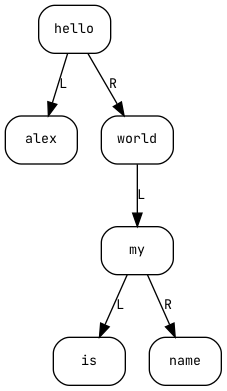
\includegraphics[height=4cm]{1639782059_16807.graph.gv}

% ---

\subsubsection{Поиск слова в ДДП: элемент найден}

\textbf{Входные данные: }
2 $\rightarrow$ my

\textbf{Слова в ДДП: }
hello, world, my, name, is, alex

\textbf{Слова в АВЛ-дереве: }
---

\textbf{Слова в хеш-таблице: }
---

\textbf{Результат: }
Слово "my" найдено в ДДП.

% ---

\subsubsection{Поиск слова в ДДП: элемент не найден}

\textbf{Входные данные: }
2 $\rightarrow$ myty

\textbf{Слова в ДДП: }
hello, world, my, name, is, alex

\textbf{Слова в АВЛ-дереве: }
---

\textbf{Слова в хеш-таблице: }
---

\textbf{Результат: }
Элемент не найден.

\subsubsection{Удаление слова из ДДП: элемент найден}

\textbf{Входные данные: }
3 $\rightarrow$ my

\textbf{Слова в ДДП: }
hello, world, my, name, is, alex

\textbf{Слова в АВЛ-дереве: }
---

\textbf{Слова в хеш-таблице: }
---

\textbf{Результат: }
Слово "my" успешно удалено из ДДП.

% ---

\subsubsection{Удаление слова из ДДП: элемент не найден}

\textbf{Входные данные: }
3 $\rightarrow$ myty

\textbf{Слова в ДДП: }
hello, world, my, name, is, alex

\textbf{Слова в АВЛ-дереве: }
---

\textbf{Слова в хеш-таблице: }
---

\textbf{Результат: }
Элемент не найден.

% ---










\subsubsection{Вывод АВЛ-дерева}

\textbf{Входные данные: }
4

\textbf{Слова в ДДП: }
---

\textbf{Слова в АВЛ-дереве: }
hello, world, my, name, is, alex

\textbf{Слова в хеш-таблице: }
---

\textbf{Результат: }

\hspace{3cm}
\includegraphics[height=4cm{1639782709_282475249.avl.graph.gv}

% ---

\subsubsection{Поиск слова в АВЛ-дереве: элемент найден}

\textbf{Входные данные: }
5 $\rightarrow$ my

\textbf{Слова в ДДП: }
---

\textbf{Слова в АВЛ-дереве: }
hello, world, my, name, is, alex

\textbf{Слова в хеш-таблице: }
---

\textbf{Результат: }
Слово "my" найдено в АВЛ-дереве.

% ---

\subsubsection{Поиск слова в АВЛ-дереве: элемент не найден}

\textbf{Входные данные: }
5 $\rightarrow$ myty

\textbf{Слова в ДДП: }
---

\textbf{Слова в АВЛ-дереве: }
hello, world, my, name, is, alex

\textbf{Слова в хеш-таблице: }
---

\textbf{Результат: }
Элемент не найден.

\subsubsection{Удаление слова из АВЛ-дерева: элемент найден}

\textbf{Входные данные: }
6 $\rightarrow$ my

\textbf{Слова в ДДП: }
---

\textbf{Слова в АВЛ-дереве: }
hello, world, my, name, is, alex

\textbf{Слова в хеш-таблице: }
---

\textbf{Результат: }
Слово "my" успешно удалено из АВЛ-дерева.

% ---

\subsubsection{Удаление слова из АВЛ-дерева: элемент не найден}

\textbf{Входные данные: }
6 $\rightarrow$ myty

\textbf{Слова в ДДП: }
---

\textbf{Слова в АВЛ-дереве: }
hello, world, my, name, is, alex

\textbf{Слова в хеш-таблице: }
---

\textbf{Результат: }
Элемент не найден.

% ---



















\subsubsection{Вывод хеш-таблицы}

\textbf{Входные данные: }
7

\textbf{Слова в ДДП: }
---

\textbf{Слова в АВЛ-дереве: }
---

\textbf{Слова в хеш-таблице: }
hello, world, my, name, is, alex

\textbf{Результат: }

\begin{minted}{text}
0000: "hello"
0001: EMPTY
0002: EMPTY
0003: "is"
0004: "name"
0005: EMPTY
0006: "world"
0006: "my"
0006: "alex"
\end{minted}


% ---

\subsubsection{Поиск слова в хеш-таблице: элемент найден}

\textbf{Входные данные: }
8 $\rightarrow$ my

\textbf{Слова в ДДП: }
---

\textbf{Слова в АВЛ-дереве: }
---

\textbf{Слова в хеш-таблице: }
hello, world, my, name, is, alex

\textbf{Результат: }
Слово "my" найдено в хеш-таблице.

% ---

\subsubsection{Поиск слова в хеш-таблице: элемент не найден}

\textbf{Входные данные: }
8 $\rightarrow$ myty

\textbf{Слова в ДДП: }
---

\textbf{Слова в АВЛ-дереве: }
---

\textbf{Слова в хеш-таблице: }
hello, world, my, name, is, alex

\textbf{Результат: }
Элемент не найден.

\subsubsection{Удаление слова из хеш-таблицы: элемент найден}

\textbf{Входные данные: }
9 $\rightarrow$ my

\textbf{Слова в ДДП: }
---

\textbf{Слова в АВЛ-дереве: }
---

\textbf{Слова в хеш-таблице: }
hello, world, my, name, is, alex

\textbf{Результат: }
Слово "my" успешно удалено из хеш-таблицы.

% ---

\subsubsection{Удаление слова из хеш-таблицы: элемент не найден}

\textbf{Входные данные: }
9 $\rightarrow$ myty

\textbf{Слова в ДДП: }
---

\textbf{Слова в АВЛ-дереве: }
---

\textbf{Слова в хеш-таблице: }
hello, world, my, name, is, alex

\textbf{Результат: }
Элемент не найден.

% ---


\subsubsection{Измерения скорости}

\textbf{Входные данные: }
10 $\rightarrow$ 100 $\rightarrow$ 150

\textbf{Слова в ДДП: }
---

\textbf{Слова в АВЛ-дереве: }
---

\textbf{Слова в хеш-таблице: }
---

\textbf{Результат: }

\begin{minted}{text}
ДДП:
  Поиск: 25, количество сравнений: 100
  Удаление: 23, количество сравнений: 100
АВЛ-дерево:
  Поиск: 1, количество сравнений: 7
  Удаление: 1, количество сравнений: 7
Хеш-таблица:
  Поиск: 0, количество сравнений: 1
  Удаление: 1, количество сравнений: 1
Файл:
  Поиск: 302, количество сравнений: 100
  Удаление: 42571, количество сравнений: 100
\end{minted}


% ---

\subsubsection{Измерения объема памяти}

\textbf{Входные данные: }
11 $\rightarrow$ 100 $\rightarrow$ 150

\textbf{Слова в ДДП: }
---

\textbf{Слова в АВЛ-дереве: }
---

\textbf{Слова в хеш-таблице: }
---

\textbf{Результат: }

\begin{minted}{text}
ДДП:
  Размер: 28000 Б
АВЛ-дерево:
  Размер: 28000 Б
Хеш-таблица:
  Размер: 28424 Б
Текстовый файл:
  Размер: 25700 Б
\end{minted}


\newpage

\section{Оценка эффективности}
\subsection{Объем занимаемой памяти}


\begin{tabular}{ |l|l|r|r|r|r| }
\hline
\textbf{Размер} & \textbf{Емкость} & \textbf{ДДП, Б} & \textbf{АВЛ-дерево, Б} & \textbf{Хеш-табл., Б} & \textbf{Файл, Б} \\ \hline
20 & 10 & 5600 & 5600 & 5544 & 5140 \\ \hline
20 & 20 & 5600 & 5600 & 5624 & 5140 \\ \hline
20 & 40 & 5600 & 5600 & 5784 & 5140 \\ \hline
200 & 100 & 56000 & 56000 & 55224 & 51400 \\ \hline
200 & 200 & 56000 & 56000 & 56024 & 51400 \\ \hline
200 & 400 & 56000 & 56000 & 57624 & 51400 \\ \hline
1000 & 500 & 280000 & 280000 & 276024 & 257000 \\ \hline
1000 & 1000 & 280000 & 280000 & 280024 & 257000 \\ \hline
1000 & 2000 & 280000 & 280000 & 288024 & 257000 \\ \hline
\end{tabular}

\subsection{Скорость операций}

\subsubsection{Поиск}

\begin{tabular}{ |l|l|r|r|r|r| }
\hline
\textbf{Размер} & \textbf{Емкость} & \textbf{ДДП} & \textbf{АВЛ} & \textbf{Хеш-таблица} & \textbf{Файл} \\ \hline
20 & 10 & 1554 & 369 & 324 & 31656 \\ \hline
20 & 20 & 1859 & 353 & 471 & 28781 \\ \hline
20 & 40 & 802 & 640 & 332 & 30627 \\ \hline
200 & 100 & 15278 & 379 & 572 & 128379 \\ \hline
200 & 200 & 9105 & 371 & 317 & 111428 \\ \hline
200 & 400 & 16723 & 519 & 199 & 128862 \\ \hline
1000 & 500 & 42754 & 441 & 281 & 357513 \\ \hline
1000 & 1000 & 40975 & 458 & 488 & 317712 \\ \hline
1000 & 2000 & 41697 & 766 & 549 & 284568 \\ \hline
\end{tabular}

\subsubsection{Удаление}

\begin{tabular}{ |l|l|r|r|r|r| }
\hline
\textbf{Размер} & \textbf{Емкость} & \textbf{ДДП} & \textbf{АВЛ} & \textbf{Хеш-таблица} & \textbf{Файл} \\ \hline
20 & 10 & 1380 & 348 & 454 & 440309 \\ \hline
20 & 20 & 1695 & 580 & 499 & 419928 \\ \hline
20 & 40 & 1855 & 323 & 225 & 383716 \\ \hline
200 & 100 & 15043 & 861 & 323 & 2671087 \\ \hline
200 & 200 & 9323 & 1879 & 460 & 2741421 \\ \hline
200 & 400 & 8301 & 857 & 482 & 2625421 \\ \hline
1000 & 500 & 41334 & 672 & 463 & 12615204 \\ \hline
1000 & 1000 & 40827 & 638 & 404 & 12806856 \\ \hline
1000 & 2000 & 41045 & 541 & 374 & 13031966 \\ \hline



\end{tabular}


\subsection{Количество сравнений}

\subsubsection{Поиск}

\begin{tabular}{ |l|l|r|r|r|r| }
\hline
\textbf{Размер} & \textbf{Емкость} & \textbf{ДДП} & \textbf{АВЛ} & \textbf{Хеш-таблица} & \textbf{Файл} \\ \hline
20 & 10 & 20 & 5 & 7 & 20 \\ \hline
20 & 20 & 20 & 5 & 2 & 20 \\ \hline
20 & 40 & 20 & 5 & 1 & 20 \\ \hline
200 & 100 & 200 & 8 & 5 & 200 \\ \hline
200 & 200 & 200 & 8 & 2 & 200 \\ \hline
200 & 400 & 200 & 8 & 1 & 200 \\ \hline
1000 & 500 & 1000 & 10 & 4 & 1000 \\ \hline
1000 & 1000 & 1000 & 10 & 3 & 1000 \\ \hline
1000 & 2000 & 1000 & 10 & 6 & 1000 \\ \hline



\end{tabular}

\subsubsection{Удаление}

\begin{tabular}{ |l|l|r|r|r|r| }
\hline
\textbf{Размер} & \textbf{Емкость} & \textbf{ДДП} & \textbf{АВЛ} & \textbf{Хеш-таблица} & \textbf{Файл} \\ \hline
20 & 10 & 20 & 5 & 1 & 20 \\ \hline
20 & 20 & 20 & 5 & 1 & 20 \\ \hline
20 & 40 & 20 & 5 & 1 & 20 \\ \hline
200 & 100 & 200 & 8 & 1 & 200 \\ \hline
200 & 200 & 200 & 8 & 2 & 200 \\ \hline
200 & 400 & 200 & 8 & 1 & 200 \\ \hline
1000 & 500 & 1000 & 10 & 2 & 1000 \\ \hline
1000 & 1000 & 1000 & 10 & 1 & 1000 \\ \hline
1000 & 2000 & 1000 & 10 & 1 & 1000 \\ \hline



\end{tabular}

\newpage


\section{Контрольные вопросы}
\subsection{Что такое дерево?}
Дерево --- это нелинейная структура данных, используемая для представления иерархических связей, имеющих отношение <<один ко многим>>.

Дерево с базовым типом $Т$ определяется рекурсивно либо как пустая структура (пустое дерево), либо как узел типа $Т$ с конечным числом древовидных структур этого же типа, называемых поддеревьями.

\subsection{Как выделяется память под представление деревьев?}

Память выделяется динамически под каждый узел дерева.

\subsection{Какие стандартные операции возможны над деревьями?}

Обход дерева, вставка элемента, удаление элемента.

\subsection{Что такое дерево двоичного поиска?}

Двоичное дерево --- дерево, каждый узел которого имеет не более двух потомков.

Дерево двоичного поиска --- это такое дерево, в котором все левые потомки моложе предка, а все правые --- старше. Это свойство называется характеристическим свойством дерева двоичного поиска и выполняется для любого узла, включая корень.

\subsection{Чем отличается идеально сбалансированное дерево от АВЛ дерева?}

У АВЛ-дерева для каждого узла высота двух его поддеревьев различается не более чем на 1, а у идеально сбалансированного дерева различается количество узлов в каждом поддереве не более чем на 1.


\subsection{Чем отличается поиск в АВЛ-дереве от поиска в дереве двоичного поиска?}

Поиск в АВЛ-дереве происходит быстрее из-за примерное одинаковой высоты каждой ветви.


\subsection{Что такое хеш-таблица, каков принцип ее построения?}

Хеш-таблица --- массив, заполненный в порядке, определяемым хеш-функцией. Хеш-функция каждому ключу ставит в соответствие некоторый индекс в массиве.

\subsection{Что такое коллизии? Каковы методы их устранения?}

Коллизия --- ситуация, когда разным ключам соответствует одно значение хеш-функции.

Методы устранений коллизий:

\subsubsection{Метод цепочек (открытое хеширование)}

В случае, когда элемент таблицы с индексом, который вернула хеш-функция, уже занят, к нему присоединяется связный список. Таким образом, если для нескольких различных значений ключа возвращается одинаковое значение хеш-функции, то по этому адресу находится указатель на связанный список, который содержит все значения. Поиск в этом списке осуществляется простым перебором, так как при грамотном выборе хеш-функции любой из списков оказывается достаточно коротким.
	
\subsubsection{Открытая адресация (закрытое хеширование)}

В этом случае, если ячейка с вычисленным индексом занята, то можно просто просматривать следующие записи таблицы по порядку (с шагом 1), до тех пор, пока не будет найден ключ K или пустая позиция в таблице. При этом, если индекс следующего просматриваемого элемента определяется добавлением какого-то постоянного шага (от 1 до n), то данный способ разрешения коллизий называется линейной адресацией.

\subsection{В каком случае поиск в хеш-таблицах становится неэффективен?}

При большом количестве коллизий.

\subsection{Эффективность поиска в АВЛ деревьях, в дереве двоичного поиска и в хеш-таблицах}

В худшем случае, в ДДП сложность поиска составляет $O(n)$, в АВЛ-дереве --- $O(\log_2 n)$, в хеш-таблице с маленьким количеством коллизий --- $O(1)$. Таким образом, хеш-таблица заметно эффективнее деревьев для поиска, при условии небольшого количества коллизий.

\newpage

\section{Вывод}

Как можно убедиться по результатам измерений, хеш-таблица
 позволяет осуществлять более быстрый поиск и удаление элементов, чем деревья. В то же время, в общем случае она менее эффективна по памяти. 
 
 Если сравнивать деревья, то поиск в АВЛ-дереве происходит быстрее. Однако, удаление в нем может быть медленнее, чем в обычном двоичном дереве поиска. Это обусловлено тем, что при удалении АВЛ-дерево нуждается в дополнительной балансировке. 
 
 Также операции в АВЛ-дереве могут быть медленнее в том случае, если искомый/удаляемый элемент находятся близко к корню в обычном ДДП, а в АВЛ-дереве он находится дальше.
 
 По памяти АВЛ-дерево менее эффективно обычного ДДП, так как каждый его узел должен содержать информацию о высоте текущего поддерева. Но эта разница в потреблении памяти менее значительна, чем, например, разница в потреблении памяти деревьями и хеш-таблицей.
 
 Относительно операций поиска и удаления наихудший результат показал текстовый файл. Такой результат обусловлен последовательным доступом к файлу, а так же накладными расходами на открытие файла.
 
 Текстовый файл является наиболее эффективным в данном случае по памяти.

\newpage
\begin{thebibliography}{2}
\addcontentsline{toc}{section}{Список литературы}
\bibitem{method}
Методические рекомендации по лабораторной работе №6(\emph{http://wwwcdl.bmstu.ru/}) 
\end{thebibliography}

\end{document}
